\documentclass{suturo}

\begin{document}
    \maketitle{Vision}{13.05.2017}{}{1}{}{}{}{}

\makeatletter
\newcommand{\chapterauthor}[1]{%
  {\parindent0pt\vspace*{-47pt}%
  \linespread{2.2}\large\begin{flushright}von: #1\end{flushright}%
  \par\nobreak\vspace*{0pt}}
  \@afterheading%
}
\makeatother

\section*{Architektur und Funktion}
\chapterauthor{Alexander Haar}
Das beliefstate-Paket dient dazu sich Aktionen die der Roboter ausgeführt hat zu speichern und auf Anfrage zu ermitteln, welcher Gripper belegt ist und welche Objekte als nächstes weggeräumt werden sollen. Außerdem spawnt der Knoten die Objektkoordinatensysteme und spawnt außerdem das Mesh des Objekts.

\begin{figure}[!htb]
        \center{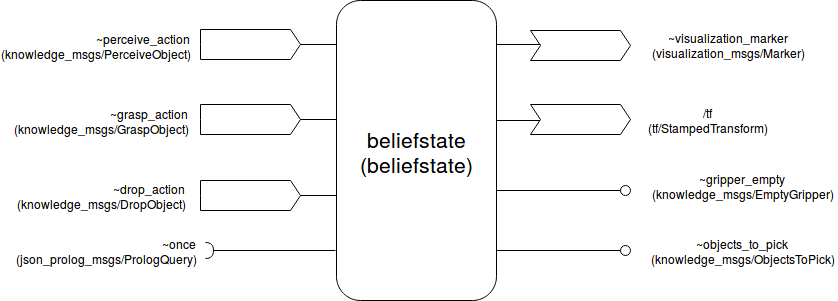
\includegraphics[width=\textwidth]
        {figures/beliefstate.png}
        \caption{\label{fig:beliefstate_node} Architektur der beliefstate-node}}
\end{figure}
      
\section*{Methodendokumentation}
\chapterauthor{Alexander Haar}

\subsection{beliefstate}

\subsubsection{to\_underscore - Python}
\begin{verbatim}
def to_underscore(name)
Beschreibung: Übersetzt einen string von Camelcase- Schreibweise 
in underscore- Schreibweise. 
@param name: Der string in Camelcase- Schreibweise.
@return: Der string in underscore- Schreibweise.
\end{verbatim}

\subsubsection{object\_url\_to\_object\_name - Python}
\begin{verbatim}
def object_url_to_object_name(url)
Beschreibung: Extrahiert aus einer Owl-Url den Namen eines Objekts.
@param url: Die Owl- Url.
@return: Der Objektname.
\end{verbatim}


\subsubsection{prolog\_query\_false - Python}
\begin{verbatim}
def prolog_query_false(query_result)
Beschreibung: Evaluiert, ob eine Prologanfrage zu false auswertet.
@param query_result: Resultat einer einer Prologanfrage.
@return: True, falls die Prologanfrage zu false evaluiert und false sonst.
\end{verbatim}

\subsubsection{prolog\_query\_true - Python}
\begin{verbatim}
def prolog_query_true(query_result)
Beschreibung: Evaluiert, ob eine Prologanfrage zu true auswertet.
@param query_result: Resultat einer einer Prologanfrage.
@return: True, falls die Prologanfrage zu true evaluiert und false sonst.
\end{verbatim}

\subsubsection{point\_to\_prolog\_list - Python}
\begin{verbatim}
def point_to_prolog_list(point)
Beschreibung: Übersetzt einen Punkt in eine Prologliste.
@param point: Der zu übersetzende Punkt.
@return: Die resultierende Prologliste.
\end{verbatim}

\subsubsection{pose\_to\_prolog\_list - Python}
\begin{verbatim}
def pose_to_prolog_list(pose)
Beschreibung: Übersetzt eine Pose in eine Prologliste.
@param pose: Die zu übersetzende Pose.
@return: Die resultierende Prologliste.
\end{verbatim}

\subsubsection{gripper\_as\_string - Python}
\begin{verbatim}
def gripper_as_string(gripper)
Beschreibung: Übersetzt eine Gripperkonstante in einen string.
@param gripper: Die zu übersetzende Gripperkonstante.
@return: Der resultierende string.
\end{verbatim}

\subsubsection{create\_query\_for\_perceive\_object - Python}
\begin{verbatim}
def create_query_for_perceive_object(perceive_object_msg)
Beschreibung: Erzeugt anhand einer PerceiveObject.msg eine Prologanfrage.
@param perceive_object_msg: Die PerceiveObject.msg.
@return: Die resultierende Prologanfrage.
\end{verbatim}

\subsubsection{create\_query\_for\_grasp\_object - Python}
\begin{verbatim}
def create_query_for_grasp_object(grasp_object_msg)
Beschreibung: Erzeugt anhand einer GraspObject.msg eine Prologanfrage.
@param grasp_object_msg: Die GraspObject.msg.
@return: Die resultierende Prologanfrage.
\end{verbatim}

\subsubsection{create\_query\_for\_drop\_object - Python}
\begin{verbatim}
def create_query_for_drop_object(drop_object_msg)
Beschreibung: Erzeugt anhand einer DropObject.msg eine Prologanfrage.
@param drop_object_msg: Die DropObject.msg.
@return: Die resultierende Prologanfrage.
\end{verbatim}

\subsubsection{create\_query\_object\_attached\_to\_gripper - Python}
\begin{verbatim}
def create_query_object_attached_to_gripper(gripper)
Beschreibung: Erzeugt anhand einer Gripperkonstante eine Prologanfrage.
@param gripper: Die Gripperkonstante.
@return: Die resultierende Prologanfrage.
\end{verbatim}

\subsubsection{object\_exists - Python}
\begin{verbatim}
def object_exists(object_class)
Beschreibung: Evaluiert, ob ein Objekt bereits wahrgenommen wurde und in 
der Wissensbasis existiert.
@param object_class: Das zu überprüfende Objekt.
@return: True, falls das Objekt in der Wissensbasis existiert und false sonst.
\end{verbatim}

\subsubsection{pose\_stamped\_to\_position\_tupel - Python}
\begin{verbatim}
def pose_stamped_to_position_tupel(pose_stamped)
Beschreibung: Übersetzt die Position eines PoseStamped in ein Tupel.
@param pose_stamped: Der zu übersetzende PoseStamped.
@return: Das resultierende Tupel.
\end{verbatim}

\subsubsection{pose\_stamped\_to\_quaternion\_tupel - Python}
\begin{verbatim}
def pose_stamped_to_quaternion_tupel(pose_stamped)
Beschreibung: Übersetzt das Quaternion eines PoseStamped in ein Tupel.
@param pose_stamped: Der zu übersetzende PoseStamped.
@return: Das resultierende Tupel.
\end{verbatim}

\subsubsection{quaternion\_to\_prolog\_list - Python}
\begin{verbatim}
def quaternion_to_prolog_list(quaternion)
Beschreibung: Übersetzt ein Quaternion in eine Prologliste.
@param quaternion: Das zu übersetzende Quaternion.
@return: Die resultierende Prologliste.
\end{verbatim}

\subsubsection{spawn\_object\_frame - Python}
\begin{verbatim}
def spawn_object_frame(object_name, object_pose)
Beschreibung: Spawnt an der angegebenen Pose ein Objektkoordinatensystem 
und das entsprechende Mesh.
@param object_name: Der Name des Objekts.
@param object_pose: Die Pose des Objekts.
\end{verbatim}

\subsubsection{update\_object\_frame - Python}
\begin{verbatim}
def update_object_frame(object_name, object_pose)
Beschreibung: Ändert die Pose des angegeben Objekts auf die übergebene.
@param object_name: Der Name des Objekts.
@param object_pose: Die Pose des Objekts.
\end{verbatim}

\subsubsection{change\_reference\_frame - Python}
\begin{verbatim}
def change_reference_frame(object_name, new_reference_frame_id)
Beschreibung: Verändert das Referenzframe des Objektkoordinatensystems 
auf das übergeben Koordinatensystem.
@param object_name: Der Name des Objekts.
@param new_reference_frame_id: Das neu Referenzkoordinatensystem.
\end{verbatim}

\subsubsection{spawn\_object\_mesh - Python}
\begin{verbatim}
def spawn_object_mesh(object_name)
Beschreibung: Spawnt ein Mesh in dem entsprechenden Objektkoordinatensystem.
@param object_name: Der Name des Objekts.
\end{verbatim}

\subsubsection{main - Python}
\begin{verbatim}
__name__ == '__main__
Beschreibung: Startet alle Service- Server und Subscriber die dieser Knoten benötigt.
\end{verbatim}

\subsubsection{object\_exists - Prolog}
\begin{verbatim}
object_exists(ObjectClass)
Beschreibung: Prüft, ob ein Individual dieser Klasse bereits in der
Wissensbasis vorhanden ist
@param ObjectClass: Die zu prüfende Objektklasse.
\end{verbatim}

\subsubsection{process\_perceive\_action - Prolog}
\begin{verbatim}
process_perceive_action(ObjectClass, PoseList, ReferenceFrame)
Beschreibung: Fügt ein Individual der Objektklasse an der angegebenen 
Pose im Referenzframe hinzu.
@param ObjectClass: Die Klasse der hinzuzufügenden Individuals.
@param PoseList: Die Pose des Objekts als Liste.
@param ReferenceFrame: Das Referenzframe.
\end{verbatim}

\subsubsection{process\_grasp\_action - Prolog}
\begin{verbatim}
process_grasp_action(ObjectClass, GripperIndividual)
Beschreibung: Fügt eine GraspAction zur Wissensbasis hinzu unter 
Verwendung des angegeben Grippers und der Objektklasse.
@param ObjectClass: Die Objektklasse.
@param GripperIndividual: Linker oder rechter Gripper.
\end{verbatim}

\subsubsection{process\_drop\_action - Prolog}
\begin{verbatim}
process_drop_action(GripperIndividual)
Beschreibung: Fügt eine DropAction zur Wissensbasis hinzu unter 
Verwendung des angegeben Grippers.
@param GripperIndividual: Linker oder rechter Gripper.
\end{verbatim}

\subsubsection{object\_attached\_to\_gripper - Prolog}
\begin{verbatim}
object_attached_to_gripper(GripperIndividual, ObjectIndividual)
Beschreibung: Prüft, ob sich ein Objekt in dem angegebenen Gripper befindet.
@param GripperIndividual: Linker oder rechter Gripper.
@param ObjectIndividual: Das Objekt, welches sich im Gripper befindet.
\end{verbatim}

\subsubsection{get\_latest\_object\_pose - Prolog}
\begin{verbatim}
get_latest_object_pose(ObjectIndividual, PoseList)
Beschreibung: Gibt die zuletzt bekannte Pose des Objekts zurück.
@param ObjectIndividual: Das Objekt.
@param PoseList: Die Pose des Objekts.
\end{verbatim}

\subsubsection{get\_objects\_on\_kitchen\_island\_counter - Prolog}
\begin{verbatim}
get_objects_on_kitchen_island_counter(ObjectList)
Beschreibung: Gibt eine Liste aller Objekte die noch verteilt
werden müssen zurück.
@param ObjectList: Eine Liste aller Objekte die noch verteilt werden müssen.
\end{verbatim}

\subsubsection{get\_two\_objects\_on\_kitchen\_island\_counter\_with\_same\_storage\_place - Prolog}
\begin{verbatim}
get_two_objects_on_kitchen_island_counter_with_same_storage_place(Object1, Object2)
Beschreibung: Gibt die zwei Objekte zurück, welche als nächstes verteilt werden sollen.
@param Object1: Das erste Objekt.
@param Object2: Das zweite Objekt.
\end{verbatim}

\section*{Schnittstellen}
\chapterauthor{Alexander Haar}

\subsection*{Subscriber process\_perceive\_action}
\begin{verbatim}
def process_perceive_action(perceive_object_msg)
Beschreibung: Erstellt anhand der Message eine Prologanfrage und
sendet diese an den json_prolog- Server. 
@param perceive_object_msg: Die PerceiveObject.msg
\end{verbatim}

\subsection*{Subscriber process\_grasp\_action}
\begin{verbatim}
def process_grasp_action(grasp_object_msg)
Beschreibung: Erstellt anhand der Message eine Prologanfrage und
sendet diese an den json_prolog- Server. 
@param grasp_object_msg: Die GraspObject.msg
\end{verbatim}

\subsection*{Subscriber process\_drop\_action}
\begin{verbatim}
def process_drop_action(drop_object_msg)
Beschreibung: Erstellt anhand der Message eine Prologanfrage und
sendet diese an den json_prolog- Server. 
@param drop_object_msg: Die DropObject.msg
\end{verbatim}

\subsection*{Service Server gripper\_empty}
\begin{verbatim}
def gripper_empty(req)
Beschreibung: Die Anfrage an den Server ist leer. Zurückgegeben werden
zwei booleans, welche angeben, ob der Gripper belegt ist.
@param req: Die Anfrage an den Service.
@return: Die Antwort des Services.
\end{verbatim}

\subsection*{Service Server object\_to\_pick}
\begin{verbatim}
def objects_to_pick(req)
Beschreibung: Gibt die zwei Objekte zurück, welche als nächstes weggeräumt werden sollen.
@param req: Die Anfrage an den Service.
@return: Die Antwort des Services.
\end{verbatim}

\section*{Programmablauf}
\chapterauthor{Alexander Haar}
\subsection*{Schritt 1: Wahrnehmen mehrerer Objekte}
Es werden mehre Objekte wahrgenommen und deren Label sowie Pose wird dem beliefstate bekannt gemacht.

\subsection*{Schritt 2: Welche zwei Objekte sollen weggeräumt werden?}
Nachdem Alle zu verteilenden Objekte bekannt sind, werden möglichst zwei Objekte ausgewählt, welche den gleichen Lagerplatz besitzen.

\subsection*{Schritt 3: Greifen eines Objekts}
Das erste der beiden Objekte wird gegriffen.

\subsection*{Schritt 4: Greifen eines weiteren Objekts}
Anschließend wird das zweite Objekt gegriffen.

\subsection*{Schritt 5: Abstellen des 1. Objekts}
Der Roboter fährt zum entsprechenden Lagerplatz und stellt es dort ab.

\subsection*{Schritt 6: Anfrage welcher der Gripper belegt ist}
Nun wird geprüft, ob beide Gripper leer sind, dies ist nicht der Fall.

\subsection*{Schritt 7: Abstellen des 2. Objekts}
Der Roboter fährt zum nächsten Lagerplatz und stellt das zweite Objekt dort ab.

\subsection*{Schritt 8: Anfrage welcher der Gripper belegt ist}
Erneut wird geprüft, ob beide Gripper leer sind, dies ist jetzt der Fall.

\subsection*{Schritt 9: Welche Objekte sollen weggeräumt werden?}
Nun beginnt dieser Prozess wieder bei Schritt 2.
\end{document}
